\documentclass{sigplanconf}
\usepackage[1stsubmission]{oopsla2016}

% The following oopsla2015 options are available:
%
% 1stsubmission   For the initial submission
% 2ndsubmission   For the 2nd submission
% final           For camera-ready

\usepackage{amsmath,amssymb,amsopn,amsthm}
\usepackage{mathtools}
\usepackage[T1]{fontenc}
\usepackage{algorithmicx,algorithm}
\usepackage[noend]{algpseudocode}
\usepackage{multirow}
\usepackage{cleveref}
\usepackage{graphicx}
\usepackage[usenames,dvipsnames]{xcolor}
\usepackage{verbatim}
\usepackage{relsize}
\usepackage{ifluatex}
\usepackage{xspace}

\usepackage{tikz}
\usetikzlibrary{fit,positioning,patterns,shapes,shapes.multipart}
\usepackage{pgfplots}
\usepackage{pgfplotstable}
\pgfplotsset{compat=1.12} 

\usepackage{courier}            % standard fixed width font
\usepackage[scaled]{helvet} % see www.ctan.org/get/macros/latex/required/psnfss/psnfss2e.pdf
\usepackage{xspace}
\usepackage{proof}
\usepackage{graphicx}
\usepackage{amsmath}
\usepackage{amsthm}
\usepackage{amscd}
\usepackage{amssymb}
\usepackage{float}
\usepackage{epsfig}
\usepackage{xcolor}
\usepackage{color}
%\usepackage{appendix}


% use latin modern font
\usepackage[T1]{fontenc}
%\usepackage{lmodern}
\usepackage[kerning,spacing]{microtype}
 
%\floatstyle{boxed}
%\restylefloat{figure}

\newcommand{\hide}[1]{} 
\newcommand{\C}[1]{\lstinline!#1!}
\newcommand {\spc}{\hspace{3pt}}
\newcommand{\spmd}{\textsc{spmd}}
\newcommand{\cegis}{\textsc{cegis}}
\newcommand{\Sk}{\textsc{Sketch}}
\newcommand{\lang}{\textsc{SyntRec}}
\newcommand{\constr}{\textsc{guc}}
\hyphenation{spmd cegis Sketch MSL Jacobi}

\newcommand{\constraintenv}{\Sigma}
\newcommand{\cfun}{\gamma}
%%% Inference rule things.
\newcommand{\integ}{\mbox{\texttt{int}}}
%%%%%%%%%%%%%%%%%%%%%%%%%%%%%%%%%%%%%%%%%%%
% Macros for the semantics
%%%%%%%%%%%%%%%%%%%%%%%%%%%%%%%%%%%%%%%%%%%

\newcommand{\valEnv}{\Sigma}
\newcommand{\typeEnv}{\Gamma}
\newcommand{\cdeclEnv}{\Pi}
\newcommand{\cEnv}{\Lambda}

%%%%%%%%%%%%%%%%%%%%%%%%%%%%%%%%%%%%%%%%%%%
%%%%%%%%%%%%%%%%%%%%%%%%%%%%%%%%%%%%%%%%%%

\newcommand{\etal}{\textit{et al.}\@\xspace}
\newcommand{\eg}{\textit{e.g.}\@\xspace}
\newcommand{\ie}{\textit{i.e.}\@\xspace}

% References
%
%\newtheorem{thm}{Theorem}
\newtheorem{lem}{Lemma}
\newtheorem{prop}{Property}

\newcommand{\thmlabel}[1]{\label{thm:#1}}
\newcommand{\thmref}[1]{Theorem~\ref{thm:#1}}
\newcommand{\lemlabel}[1]{\label{lem:#1}}
\newcommand{\lemref}[1]{Lemma~\ref{lem:#1}}

\newcommand{\corlabel}[1]{\label{cor:#1}}
\newcommand{\corref}[1]{Corollary~\ref{cor:#1}}

\newcommand{\proplabel}[1]{\label{prop:#1}}
\newcommand{\propref}[1]{Proposition~\ref{prop:#1}}
\newcommand{\deflabel}[1]{\label{def:#1}}
\newcommand{\defref}[1]{Definition~\ref{def:#1}}
\newcommand{\exlabel}[1]{\label{ex:#1}}
\newcommand{\exref}[1]{Example~\ref{ex:#1}}
\newcommand{\problabel}[1]{\label{prob:#1}}
\newcommand{\probref}[1]{Problem~\ref{prob:#1}}
\newcommand{\obslabel}[1]{\label{obs:#1}}
\newcommand{\obsref}[1]{Observation~\ref{obs:#1}}
\newcommand{\alglabel}[1]{\label{alg:#1}}
\newcommand{\algref}[1]{Algorithm~\ref{alg:#1}}
%
\newcommand{\applabel}[1]{\label{app:#1}}
\newcommand{\appref}[1]{Appendix~\ref{app:#1}}
\newcommand{\seclabel}[1]{\label{sec:#1}}
\newcommand{\shortsecref}[1]{\S\ref{sec:#1}}
\newcommand{\longsecref}[1]{Section~\ref{sec:#1}}
%
\newcommand{\tablabel}[1]{\label{tab:#1}}
\newcommand{\tabref}[1]{Table~\ref{tab:#1}}
\newcommand{\figlabel}[1]{\label{fig:#1}}
\newcommand{\longfigref}[1]{Figure~\ref{fig:#1}}
\newcommand{\shortfigref}[1]{Fig.~\ref{fig:#1}}
\newcommand{\eqqlabel}[1]{\label{eq:#1}}
\newcommand{\shorteqqref}[1]{\eqref{eq:#1}}
\newcommand{\mediumeqqref}[1]{Eq.~\eqref{eq:#1}}
\newcommand{\longeqqref}[1]{Equation~\eqref{eq:#1}}

% Determine type of references for particular document.
%
\newcommand{\secref}{\longsecref}
\newcommand{\figref}{\longfigref}
\newcommand{\eqqref}{\longeqqref}

% Numbering layout
%
\numberwithin{equation}{section}
\newtheorem{definition}{Definition}
\newtheorem{corollary}{Corollary}
\newtheorem{hypothesis}{Hypothesis}
\newtheorem{algo}{Algorithm}
\newtheorem{Equation}{Equation}
\newtheorem{theorem}{Theorem}[section]


                     %%% Commands for formatting code %%%


% \token -- used for a literal code token
% \nterm -- used for a grammar non-terminal
% Example:  Every \nterm{AssertStmt} begins with the \token{assert} keyword.
\newcommand{\token}[1]{\code{#1}}
\newcommand{\formatnt}[1]{{\sl#1}}  % This _must_ be {\sl#1}, not \textsl{#1}
\newcommand{\nterm}[1]{\index{#1@\formatnt{#1}}\formatnt{#1}}

% syntax -- environment for specifiying syntax
\newenvironment{syntax}
 {\par\begin{tabular}{rcl}}
 {\end{tabular}\vspace{2ex}}

% \lexrule -- used to define a lexical regexp rule within a syntax environment
% Example:  \lexrule{IntegerLiteral}{[0-9]+}
\newcommand{\lexrule}[2]
 {\index{#1@\formatnt{#1}|defpage}\formatnt{#1} &
  $=$ & $\langle${\tt#2}$\rangle$ \\}

% \grammar -- used to define a grammar non-terminal within a syntax environment
% \grammaralt -- used for alternate definitions within a syntax environment
% Example:  \grammar{Expr}{\nterm{Expr} \token{+} \nterm{Expr}}
%           \grammaralt{\token{(} \nterm{Expr} \token{)}}
\newcommand{\grammar}[2]
 {\index{#1@\formatnt{#1}|defpage}\formatnt{#1} & $=$ & {#2} \\}
\newcommand{\grammaralt}[1]{& $|$ & {#1} \\}
\newcommand{\grammarelt}[2]
 {\index{#1@\formatnt{#1}|defpage}\formatnt{#1} & $\in$ & {#2} \\}

\newcommand{\galt}{\mbox{\hspace{0.7em}\ensuremath{|}\hspace{1em}}}

%%% Commands for inserting special characters %%%

% \bs -- used to create a monospace backslash
\newcommand{\bs}{{\tt\char"5C}}

% \us -- used to create a monospace underscore (works better than {\tt\_})
\newcommand{\us}{{\tt\char"5F}}


\usepackage[T1]{fontenc}
%\usepackage[scaled=0.85]{luximono}


\definecolor{dkgreen}{rgb}{0,0.3,0}
\definecolor{gray}{rgb}{0.5,0.5,0.5}
\definecolor{mauve}{rgb}{0.58,0,0.82}
\definecolor{light-gray}{gray}{0.80}

\usepackage{listings}
\lstdefinelanguage{sketch}{
  morekeywords = {
       bool, harness, data, int, bool, adt, new, return, assert , case, switch},
  morecomment=[s]{/*}{*/},
}


\lstset{
  language=sketch,
  columns=flexible,
  basicstyle=\fontfamily{lmss}\selectfont\small,
  numbers=none,
  numbersep=3pt,
  numberstyle=\tiny,
  stepnumber=1,
  tabsize=2,
  breaklines=false,
  breakatwhitespace=true,
  commentstyle=\color{cyan},
  mathescape=true,
  escapeinside={\%*}{*)}
}




\renewcommand{\scriptsize}{\fontsize{8.5}{9}\selectfont}
\makeatletter
\lst@AddToHook{TextStyle}{\let\lst@basicstyle\scriptsize\fontfamily{lmss}\selectfont}
\makeatother

\usepackage{url}

\newcommand{\pr}[1]{\left(#1\right)}
\renewcommand{\t}[1]{\text{#1}}
\renewcommand{\b}[1]{\t{\lstinline{#1}}}
\newcommand{\msc}[1]{\ensuremath{\text{{\texttt{#1}}}}}
%\renewcommand{\hss}{\hspace{\stretch{1}}}
\renewcommand{\vss}{\vspace{10pt}}
\newcommand{\sem}[1]{[\![#1]\!]}
\newcommand{\esem}[1]{\mathcal{E}[\![#1]\!]}
\newcommand{\tsem}[1]{\mathcal{T}[\![#1]\!]}
\newcommand{\lam}[2]{\ensuremath{\lambda #1 .\hspace{0.01em} #2}}
\newcommand{\allq}[2]{\ensuremath{\forall #1 .\hspace{0.01em} #2}}
\newcommand{\dbr}[2]{\ensuremath{\{\hspace{-0.2em}| \,#1\,|\,#2\, |\hspace{-0.2em}\}}}
\newcommand{\secsp}{\vspace*{20pt}}

\newcommand{\csubtype}{<:_c}
\newcommand{\fsubtype}{<:_f}
\newcommand{\lub}{\sqcup}
\newcommand{\biglub}{\bigsqcup}
\newcommand{\guard}{\mathcal{G}}

\newcommand{\tenv}{\Gamma}
\newcommand{\denv}{\Delta}
\newcommand{\cenv}{\Sigma}

\newcommand{\stack}[2]{\genfrac{}{}{0pt}{0}{#1}{#2}}

\newcommand{\ors}{\ensuremath{\ |\ \ }}
\newcommand{\deriv}[5]{#1 \vdash \langle #2, #3 \rangle \rightarrow \langle #4, #5 \rangle}
\newcommand{\derivstar}[5]{#1 \vdash \langle #2, #3 \rangle \rightarrow^* \langle #4, #5 \rangle}
\newcommand{\tcrule}[3]{#1 \vdash^c #2 : #3 }
\newcommand{\tdrule}[3]{#1 \vdash #2 : #3}

\newcommand{\nrec}{\stackrel{nr}{\rightarrow}}

% Variables used in symantics and proofs.
\newcommand{\cprim}{c}
\newcommand{\constraint}{\gamma}
\newcommand{\model}{\msc{Model}}
\newcommand{\symbolic}{\sigma}
\newcommand{\store}{\sigma}
\newcommand{\irreducible}{\upsilon}
\newcommand{\levels}{\mathcal{L}}
\newcommand{\lorder}{\sqsubseteq_\levels}
\newcommand{\unsat}{\msc{Unsat}}
\newcommand{\translatesto}{\hookrightarrow}

% For properties...
\newcommand{\spair}[3]{\langle #1 | #2 \rangle_#3}
\newcommand{\cproj}[3]{[#1]_{#2, #3}}

\newcommand{\basetype}{\beta}
\newcommand{\typair}[2]{\langle #1, #2 \rangle}

\def\Cpp{C{}\texttt{++}~}





















\usepackage{rotating}

\usepackage{enumitem}
%\usepackage[breaklinks]{hyperref}

%%\hypersetup{pdfborder={0 0 100}}
%%\usepackage[hyphens]{url}

\newcommand{\lstc}[1]{\text{\lstinline{#1}}}

%\newtheorem{theorem}{Theorem}[section]
\newtheorem{lemma}[theorem]{Lemma}
\newtheorem{proposition}[theorem]{Proposition}
%\newtheorem{corollary}[theorem]{Corollary}
%\newtheorem{definition}[theorem]{Definition}
\newtheorem{example}[theorem]{Example}


\newcommand{\code}[1]{\textsf{#1}}

\newcommand{\conf}[1]{}
\newcommand{\techrep}[1]{#1}

\newcommand{\Mona}{\textsc{Mona}\xspace}

%\newcommand{\Dryad}{\textsc{Dryad}$_\textrm{sep}$\xspace}
%\newenvironment{proof}[1][Proof]{\begin{trivlist}
%\item[\hskip \labelsep {\bfseries #1}]}{\end{trivlist}}
\newcommand{\dryadtree}{\textsc{Dryad}$_\textrm{tree}$\xspace}
\newcommand{\Dryaddec}{\textsc{Dryad}$^\textrm{dec}_\textrm{tree}$\xspace}

%\newcommand{\head}{{\tt head}\xspace}
%\newcommand{\tail}{{\tt tail}\xspace}
%\newcommand{\rroot}{{\tt root}\xspace}
%\newcommand{\nnext}{{\tt next}\xspace}
%\newcommand{\pprev}{{\tt prev}\xspace}
%\newcommand{\loglisthead}{{\tt log\_listhead}\xspace}
%\newcommand{\chname}{{\tt chname}\xspace}
%\newcommand{\filename}{{\tt filename}\xspace}
%\newcommand{\data}{{\tt data}\xspace}

\newcommand{\error}{{\textit{error}}\xspace}
\newcommand{\ffalse}{{{\tt false}}\xspace}
\newcommand{\ttrue}{{{\tt true}}\xspace}
\newcommand{\f}{{\textit{f}}\xspace}
\newcommand{\g}{{\textit{g}}\xspace}


\newcommand{\Dryad}{{\sc Dryad}\xspace}

\newcommand{\head}{{\tt head}\xspace}
\newcommand{\tail}{{\tt tail}\xspace}
\newcommand{\rroot}{{\tt root}\xspace}
\newcommand{\nnext}{{\tt next}\xspace}
\newcommand{\pprev}{{\tt prev}\xspace}
\newcommand{\loglisthead}{{\tt log\_listhead}\xspace}
\newcommand{\chname}{{\tt chname}\xspace}
%\newcommand{\filename}{{\tt filename}\xspace}
\newcommand{\data}{{\tt data}\xspace}
\newcommand{\stmt}{{\tt Stmt}\xspace}
\newcommand{\strfields}{{F}\xspace}

\newcommand{\st}{{\textit st}}
\newcommand{\equal}{{\textit{equal}}}
\newcommand{\dt}{{\textit{dt}}}
\newcommand{\Nadapt}{{\textit Nadapt}}


\newcommand{\adapt}{{\textit{adapt}}}
\newcommand{\Active}{{\textit{active}}}
\newcommand{\nilnode}{{\textit{xnil}}}
\newcommand{\nil}{{\textit{nil}}}
\newcommand{\niltt}{\texttt{nil}\xspace}
\newcommand{\Assume}{{\texttt{assume}}}

\newcommand{\h}{{\textit{h}}}
\newcommand{\rr}{{\textit{r}}}
\newcommand{\p}{{\textit{p}}}
\newcommand{\q}{{\textit{q}}}
\newcommand{\z}{{\textit{z}}}
\newcommand{\x}{{\textit{x}}}
\newcommand{\y}{{\textit{y}}}
\newcommand{\ex}{{\textit{ex}}}
\newcommand{\new}{{\textit{new}}}
\newcommand{\newnode}{{\textit{new}}}
\newcommand{\free}{{\textit{free}}}
\newcommand{\nilvar}{{\textit{nil}}}
\newcommand{\undefined}{{\textit{ndef}}}
\newcommand{\Var}{{\textit{Var}}}

\renewcommand{\implies}{\Rightarrow}

\newcommand{\tuple}[1]{\langle #1 \rangle}
%\newcommand{\ignore}[1]{}
\newcommand{\pc}{\textit{pc}}
\newcommand{\Goal}{\mbox{\textit{Target}}}
\newcommand{\Loc}{\textit{Local}}
\newcommand{\G}{\textit{Global}}
\newcommand{\PC}{\textit{PC}}
\newcommand{\Params}{\mbox{\textit{Par}}}
\newcommand{\atomic}{\mbox{\textit{atom}}}

\newcommand{\calP}{{\cal P}}
\newcommand{\eager}{\mbox{Eager}}
%\newcommand{\qed}{\hfill \mbox{\raggedright \rule{.07in}{.1in}}}

\newcommand{\Strand}{{\sc Strand}\xspace}
\newcommand{\Stranddecsem}{{\sc Strand}\ensuremath{_\textit{dec}^\textit{sem}}\xspace}
\newcommand{\Stranddec}{{\sc Strand}\ensuremath{_\textit{dec}^\textit{syn}}\xspace}
\newcommand{\Stranddecbold}{{\bfseries\scshape Strand}\ensuremath{_\textit{\bfseries dec}^\textit{\bfseries sem}}}
\newcommand{\Stranddecsyn}{{\sc Strand}\ensuremath{_\textit{dec}^\textit{syn}}\xspace}
\newcommand{\Stranddecsynbold}{{\scshape \bfseries Strand}\ensuremath{_\textit{\bfseries dec}}}
\newcommand{\Stranddectree}{{\sc Strand}\ensuremath{_\textit{dec}^{\textit{tree}}}}
\newcommand{\ValidSubmodel}{\textit{ValidSubModel}}
\newcommand{\Subtree}{\textit{Subtree}}
\newcommand{\Graph}{\textit{Graph}}

\newcommand{\SH}{\textit{SH}}
\newcommand{\df}{\textit{df}}
\newcommand{\edf}{f}
\newcommand{\DF}{\textit{DF}}
\newcommand{\pv}{\textit{pv}}
\newcommand{\PV}{\textit{PV}}
\newcommand{\pre}{\textit{pre}}
\newcommand{\post}{\textit{post}}
\newcommand{\dir}{\textit{dir}}
\newcommand{\edir}{d}
\newcommand{\Dir}{\textit{PF}}
\newcommand{\FP}{\textit{F\!P}}
\newcommand{\old}{\textit{old}}
\newcommand{\Def}{\textit{Def}}
\newcommand{\base}{\textit{base}}
\newcommand{\ind}{\textit{ind}}
\newcommand{\aexpr}{\textit{aexpr}}
\newcommand{\bexpr}{\textit{bexpr}}
\newcommand{\TS}{\textit{T\!S}}
\newcommand{\ts}{\textit{ts}}
\newcommand{\Cc}{{C^c}}
\newcommand{\ccnil}{{c_{\textit nil}^c}}
\newcommand{\dirc}{{\textit{dir}^c}}
\newcommand{\dfc}{{\textit{df}^c}}
\newcommand{\pvc}{{\textit{pv}^c}}

\newcommand{\expand}{\textit{expand}}
\newcommand{\funrestrict}[2]{{#1} \mid_{#2}}
\newcommand{\funsubst}[3]{{#1}[{#2} \leftarrow {#3}]}
\newcommand{\formsubst}[3]{{#1}[{#2} / {#3}]}


\newcommand{\key}{\textit{key}}
\newcommand{\keys}{\textit{keys}}
\newcommand{\bst}{\textit{bst}}
\newcommand{\LEFT}{\textit{left}}
\newcommand{\RIGHT}{\textit{right}}

\newcommand{\pf}{\textit{pf}}
\newcommand{\PF}{\textit{PF}}
\newcommand{\vect}[1]{\,\overrightarrow{\!\!#1}}
\newcommand{\ret}{\textit{ret}}
\newcommand{\precall}{\textit{pre\_call}}
\newcommand{\postcall}{\textit{post\_call}}
\newcommand{\precallName}[1]{\textit{pre\_call}\_{#1}}
\newcommand{\postcallName}[1]{\textit{post\_call}\_{#1}}
\newcommand{\vc}{\textit{vc}}
\newcommand{\reachNodes}{\textit{reach\_nodes}}
\newcommand{\treeNodes}{\textit{tree\_nodes}}
%\newcommand{\fresh}[1]{{#1}_\textit{fresh}}
\newcommand{\fresh}[1]{\textit{fresh}\_{#1}}
\newcommand{\oldName}[1]{{#1}_\textit{old}}

\newcommand{\scope}{\text{scope}}
\newcommand{\heapless}{\text{pure}}
\newcommand{\reach}{\text{reachset}}
\newcommand{\tight}{\text{dom-ext}}


\newcommand{\Deref}{\textit{Deref}}
\newcommand{\Mod}{\textit{Mod}}
\newcommand{\Call}{\textit{Call}}
\newcommand{\Return}{\textit{Return}}
\newcommand{\footprint}{\textit{fp}}
\newcommand{\rec}{\textit{rec}}


\newcommand{\assume}{\texttt{assume }}
\newcommand{\assert}{\texttt{assert }}
\newcommand{\fpre}{\varphi_\textit{pre}}
\newcommand{\fpost}{\varphi_\textit{post}}
%\newcommand{\nil}{\texttt{nil}}
\newcommand{\emp}{\texttt{emp}}
\newcommand{\true}{\texttt{true}}
\newcommand{\sep}{*}
\newcommand{\lf}{\textit{left}}
\newcommand{\rf}{\textit{right}}
\newcommand{\kf}{\textit{key}}
\newcommand{\rkeys}{\textit{keys}^\dlt_{\vect{\pf}}}
\newcommand{\defrkeys}{\textbf{\textit{keys}}^{\tiny\dlt}_{\tiny\vect{\pf}}}
\newcommand{\figrkeys}{\textit{keys}^{\tiny\dlt}_{\tiny\vect{\pf}}}
\newcommand{\heap}{\textit{mheap}^\dlt_{\vect{\pf}}}
\newcommand{\defheap}{\textbf{\textit{mheap}}^{\tiny\dlt}_{\tiny\vect{\pf}}}
\newcommand{\figheap}{\textit{mheap}^{\tiny\dlt}_{\tiny\vect{\pf}}}
\newcommand{\Logic}{\textsf{DRYAD}}
\newcommand{\reachex}{\textit{reach}_{\{ \lf, \rf \}}}
\newcommand{\GHpre}{G_{pre}}
\newcommand{\GHpost}{G_{post}}
\newcommand{\GH}{G}
\newcommand{\lx}{\textit{lx}}
\newcommand{\rx}{\textit{rx}}

\newcommand{\dlt}{\Delta}

\newcommand{\Stefanescu}{{\c S}tef{\u a}nescu\xspace}

\newcommand{\CopyVars}{{\mathit CopyVars}}
\newcommand{\CopyVarsExcept}{{\mathit CopyVarsExcept}}
\newcommand{\CopyStrFields}{{\mathit CopyStrFields}}
\newcommand{\CopyStrFieldsExcept}{{\mathit CopyStrFieldsExcept}}
\newcommand{\CopyActiveNodes}{{\mathit CopyActiveNodes}}
\newcommand{\CopyActiveNodesExcept}{{\mathit CopyActiveNodesExcept}}
\newcommand{\CopyDataFields}{{\mathit CopyDataFields}}
\newcommand{\CopyDataFieldsExcept}{{\mathit CopyDataFieldsExcept}}
\newcommand{\vcdryadurl}{http://www.cs.illinois.edu/~madhu/vcdryad}

\newcommand{\vcdryad}{\textsc{VCDryad}\xspace}
\newcommand{\vcc}{\textsc{Vcc}\xspace}
\newcommand{\boogie}{\textsc{Boogie}\xspace}



\begin{document}

\copyrightdata{978-1-nnnn-nnnn-n/yy/mm} 
%\doi{nnnnnnn.nnnnnnn}

% Uncomment one of the following two, if you are not going for the 
% traditional copyright transfer agreement.

%\exclusivelicense                % ACM gets exclusive license to publish, 
                                  % you retain copyright

%\permissiontopublish             % ACM gets nonexclusive license to publish
                                  % (paid open-access papers, 
                                  % short abstracts)

\title{Deriving Divide-and-Conquer Dynamic Programming Algorithms Using 
  Solver-Aided Transformations}

\authorinfo{Name1}
           {Affiliation1}
           {Email1}
\authorinfo{Name2\and Name3}
           {Affiliation2/3}
           {Email2/3}

\maketitle

\begin{abstract}
We introduce \newterm{solver-aided tactics} as a mechanism for transforming
computational terms 
in the interest of deriving better, more efficient
implementations. 
Solver-aided tactics allow us to combine deductive and constraint-based synthesis to generate provably correct efficient implementations from a very high-level specification of an algorithm by chaining together a small number of high-level transformation steps. Our solver-aided tactics also leverage a type system, which incorporates predicate abstraction to associate semantic information with program terms, to guide transformations and provide enough context for automated proofs. 

In this paper, we develop the technique in the context of a system called Bellmania that uses solver-aided tactics to derive parallel divide-and-conquer implementations of dynamic programming algorithms that have better locality and are significantly more efficient than traditional loop-based implementations. Bellmania includes a high-level language for specifying dynamic programming algorithms and a calculus that facilitates gradual transformation of these specifications into efficient implementations. In particular, it provides solver-aided tactics that formalize the divide-and-conquer technique and a visualization interface to help users to interactively guide the transformation process. 
We have used the system to generate provably correct implementations of several algorithms including some important algorithms from computational biology, and show that the performance is comparable to that of the best manually optimized code.
\end{abstract}

\category{CR-number}{subcategory}{third-level}

% general terms are not compulsory anymore, 
% you may leave them out
\terms
term1, term2

\keywords
keyword1, keyword2

\section{Introduction}
\label{intro}

\begin{center}$\vdots$\end{center}

As a motivating example, we consider the Simplified Gap problem.
An intelligent agent is given two strings $x$ and $y$, and is requested
to make them equal by deleting the characters at index range $[i..j)$
from $x$, at a cost of $w_{ij}$ ($0\leq i<j\leq |x|$), from $y$,
at a cost of $w'_{ij}$ ($0\leq i<j\leq |y|$), or by repeating these steps
an arbitrary number of times.
\footnote{In the full version of the gap problem, the agent is also allowed to replace a character $\alpha$ with a character $\beta$, at some cost $c_{\alpha\beta}$.}

The optimal cost is given by the following recurrence:

\begin{equation}
\renewcommand\arraystretch{1.5}
\begin{array}{l@{}l}
	G_{ij} ~=~  &
	\begin{cases}
		0                        & i=j=0 \\
		w_{0j}                   & i=0, j>0 \\
		w'_{i0}                  & i>0, j=0 \\
		\begin{array}{@{}l@{~}l}
		  \min\langle & \underset{0\leq q<j}\min ~ G_{iq} + w_{qj}, \\
		              & \underset{0\leq p<i}\min ~ G_{pj} + w'_{pi}~\rangle
		\end{array}              & i,j>0
	\end{cases}
\end{array}
\label{intro:gap spec}
\end{equation}

\smallskip\noindent
where the desired value is $G_{|x||y|}$.

\medskip
With standard dynamic programming, this recurrence can be computed
with an iterative program, by understanding the dependency pattern:
each value $G_{ij}$ is computed from other values $G_{i'j'}$ with lower
indexes, $i'<i$, ~$j'<j$. Therefore, considering $G$ as a two-dimensional
array, it can be filled in a single pass from left to right and from top
to bottom.

\newcommand\FORLINE[1]{\STATE\algorithmicfor~{#1} \algorithmicdo~}

\begin{algorithm}
\renewcommand\arraystretch{1.3}
\begin{algorithmic}
  \STATE $G_{00} := 0$
  \FORLINE{$j=1..|y|$}  $G_{0j} := w_{0j}$  
  \FOR{$i=1..|x|$}
    \STATE $G_{i0} := w'_{i0}$
    \FOR{$j=1..|y|$}
      \STATE $G_{ij} :=
        \begin{array}[t]{@{}l@{~}l} 
          \min\langle & \underset{0\leq q<j}\min ~ G_{iq} + w_{qj}, \\
                      & \underset{0\leq p<i}\min ~ G_{pj} + w'_{pi}~\rangle 
        \end{array}$
    \ENDFOR
  \ENDFOR
\end{algorithmic}
\end{algorithm}

The same intuition underlies the divide-and-conquer approach for making
a parallel version of the same computation. The array $G$ is partitioned into
quadrants and dependencies are observed at the level of quadrants. The same reasoning
has to be repeated at a coarser level;
so, say the quadrants are labeled 1, 2, 3, and 4, then the computations of 2 and 3 depend on 1,
and the computation of 4 depends on 2 and 3.

\newcommand\qbox[1]{\fbox{\scriptsize#1}}

\begin{figure}[b]
$\renewcommand\arraystretch{2}G ~=~
 \begin{array}{|@{\quad}c@{\quad}|@{\quad}c@{\quad}|} \hline 1 & 2 \\[1mm] \hline 3 & 4 \\[1mm] \hline\end{array}$
\qquad
$\begin{array}{l}\qbox1 \rightsquigarrow \qbox2 \\ 
\qbox1 \rightsquigarrow \qbox3 \\ \qbox2\rightsquigarrow \qbox4 \\ \qbox3 \rightsquigarrow \qbox4\end{array}$
\end{figure}

\medskip
The algorithm designer then writes the following pseudo-code:

\begin{algorithmic}[1]
  \STATE Compute \qbox1 (using only input data $w,w'$).
  \STATE Compute \qbox2 using data from \qbox1.
  \STATE Compute \qbox3 using data from \qbox1.
  \STATE Compute \qbox4 using data from \qbox2 and \qbox3.
\end{algorithmic}

We say that the computation is \newterm{stratified},
in the sense that information flows only in one direction. It can be depicted as
a sequence of steps, each of which reads some regions from the array (possibly none)
and writes into a target region. It can be viewed as a chain, like the one in
\Cref{intro:chain}.

\begin{figure}
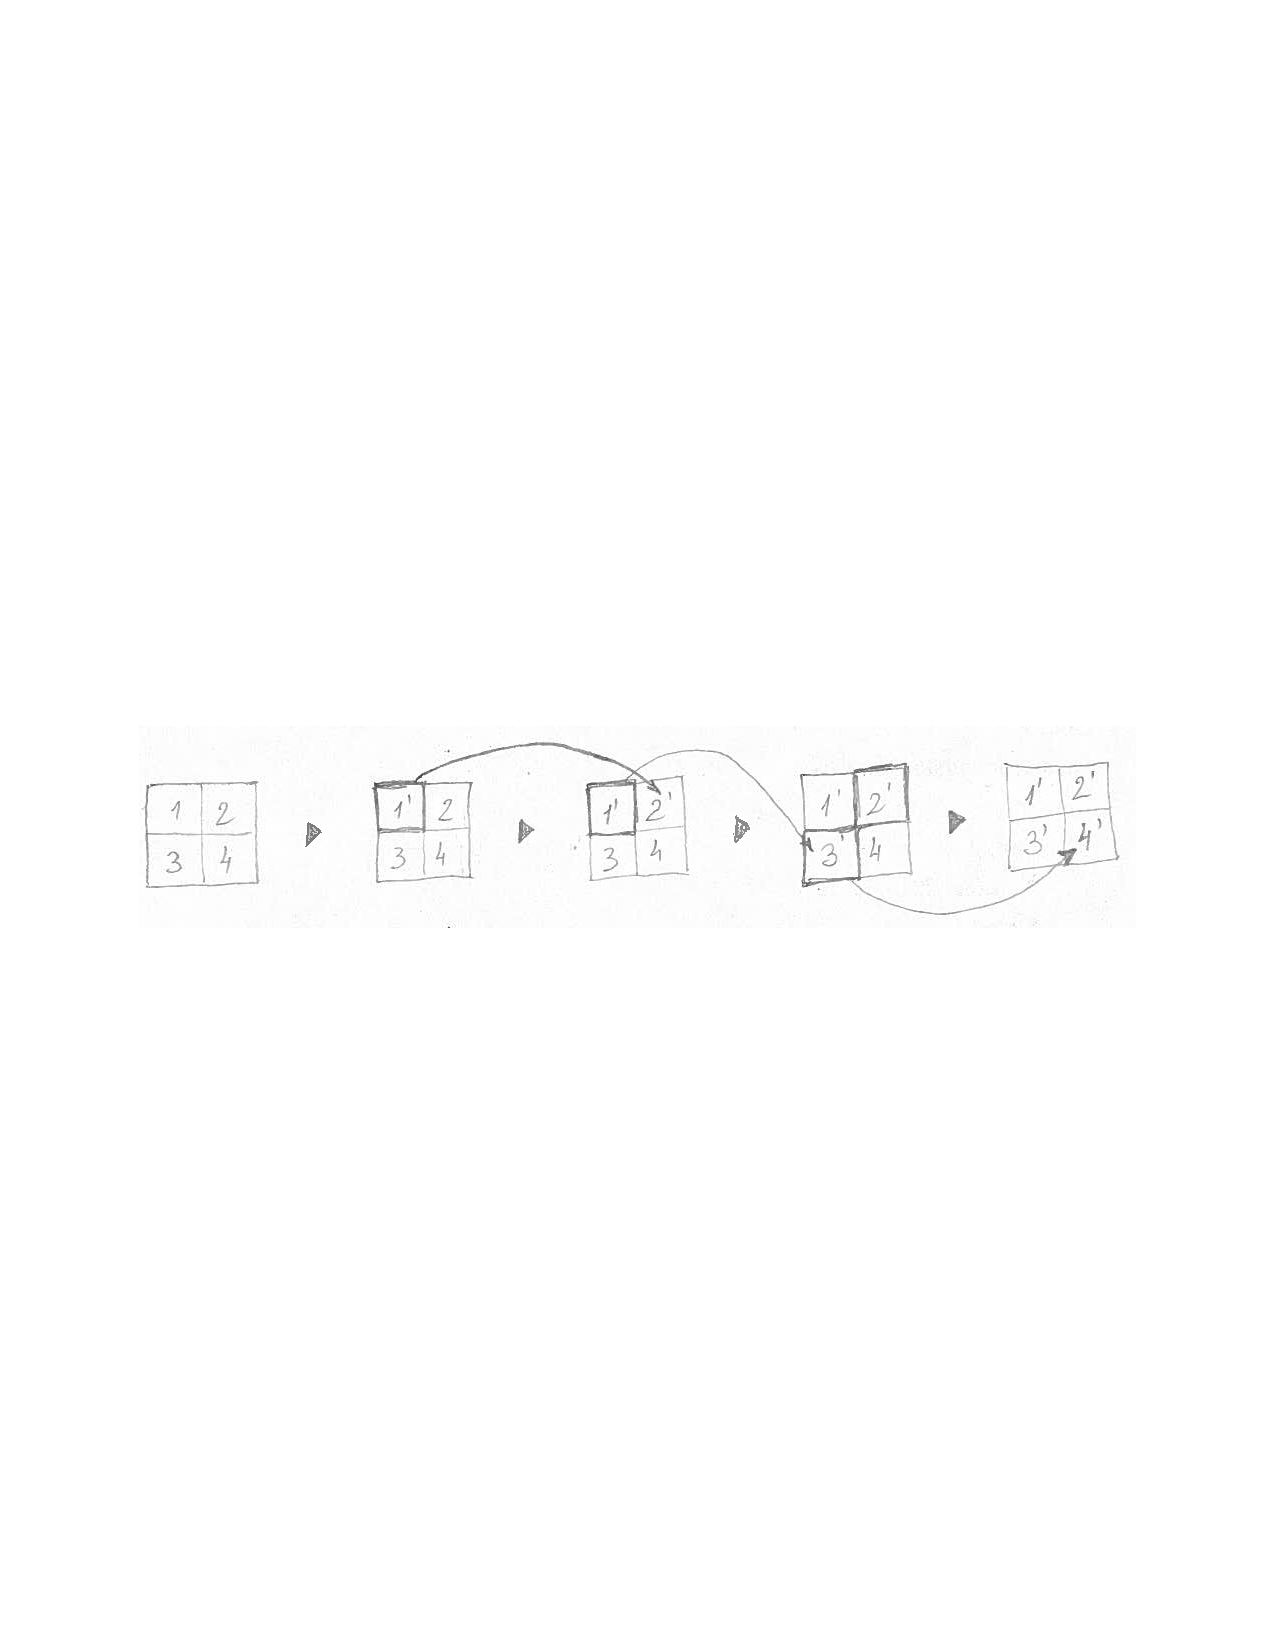
\includegraphics[width=.47\textwidth]{img/gap-stratify1}
\caption[caption]{\label{intro:chain}
  Stratified computation for Simplified Gap. \\[.2em]
  Thick borders indicate the region that is read at each step.}
\end{figure}

At this point it can be noticed that step 1 is equivalent to the original
algorithm when given as input the prefixes of $x$ and $y$ whose length correspond to the
height and width of \qbox1.

With the other three steps, however, things are not so simple:
each of them is required to process some data in addition to the input.
For example, step 2 is required to read values from \qbox1, due to the expression
$G_{iq}$ (where $\scriptstyle 0\leq q<j$).
In order to reason more formally, we define $J$ and $K$ the index sets of the rows
and columns, respectively; $J_0$, $J_1$ for the top and bottom row indexes, respectively;
and $K_0$, $K_1$ for the left and right column indexes (\Cref{intro:slice G}).
The specifications for step 2 then take the following form:

\begin{figure}
\[
\renewcommand\arraystretch{2}
\begin{array}{c|c|c|c|}
  \multicolumn{2}{c}{} & \multicolumn{2}{c}{K} \\ \cline{3-4}
  \multicolumn{2}{c}{} & \multicolumn{1}{c}{K_0}  & \multicolumn{1}{c}{K_1}\\ \cline{3-4}
  \multirow{2}{*}{$J$} & J_0 & 1 & 2 \\ \cline{3-4}
    & J_1 & 3 & 4 \\ \cline{3-4}
\end{array}
\]
\caption{\label{intro:slice G}
  Addressing quadrants in a two-dimensional array.}
\end{figure}

\makeatletter
\newcommand{\LeftEqNo}{\let\veqno\@@leqno}
\makeatother

\begin{equation}\LeftEqNo
\renewcommand\arraystretch{1.5}
\begin{array}{l@{}l}
	G_{\,(i :: J_0)\,(j :: K_1)} ~=~  \\
	\qquad
	\begin{cases}
		0                        & i=j=0 \\
		w_{0j}                   & i=0, j>0 \\
		w'_{i0}                  & i>0, j=0 \\
		\begin{array}{@{}l@{~}l}
		  \min\langle & \underset{0\leq (q::K) <j}\min ~ G_{iq} + w_{qj}, \\
		              & \underset{0\leq (p::J_0) <i}\min ~ G_{pj} + w'_{pi}~\rangle
		\end{array}              & i,j>0
	\end{cases}
\end{array}
\end{equation}

\medskip
Type annotations have been placed on $i$, $j$, $p$, and $q$ to define the regions
over which they range. $i::J_0, j::K_1$ means that the element $G_{ij}$
is always in \qbox2. Similarly, $G_{pj}$ is also in \qbox2. $G_{iq}$ is either in
\qbox1 or in \qbox2.

\begin{figure}
\begin{tabular}{l}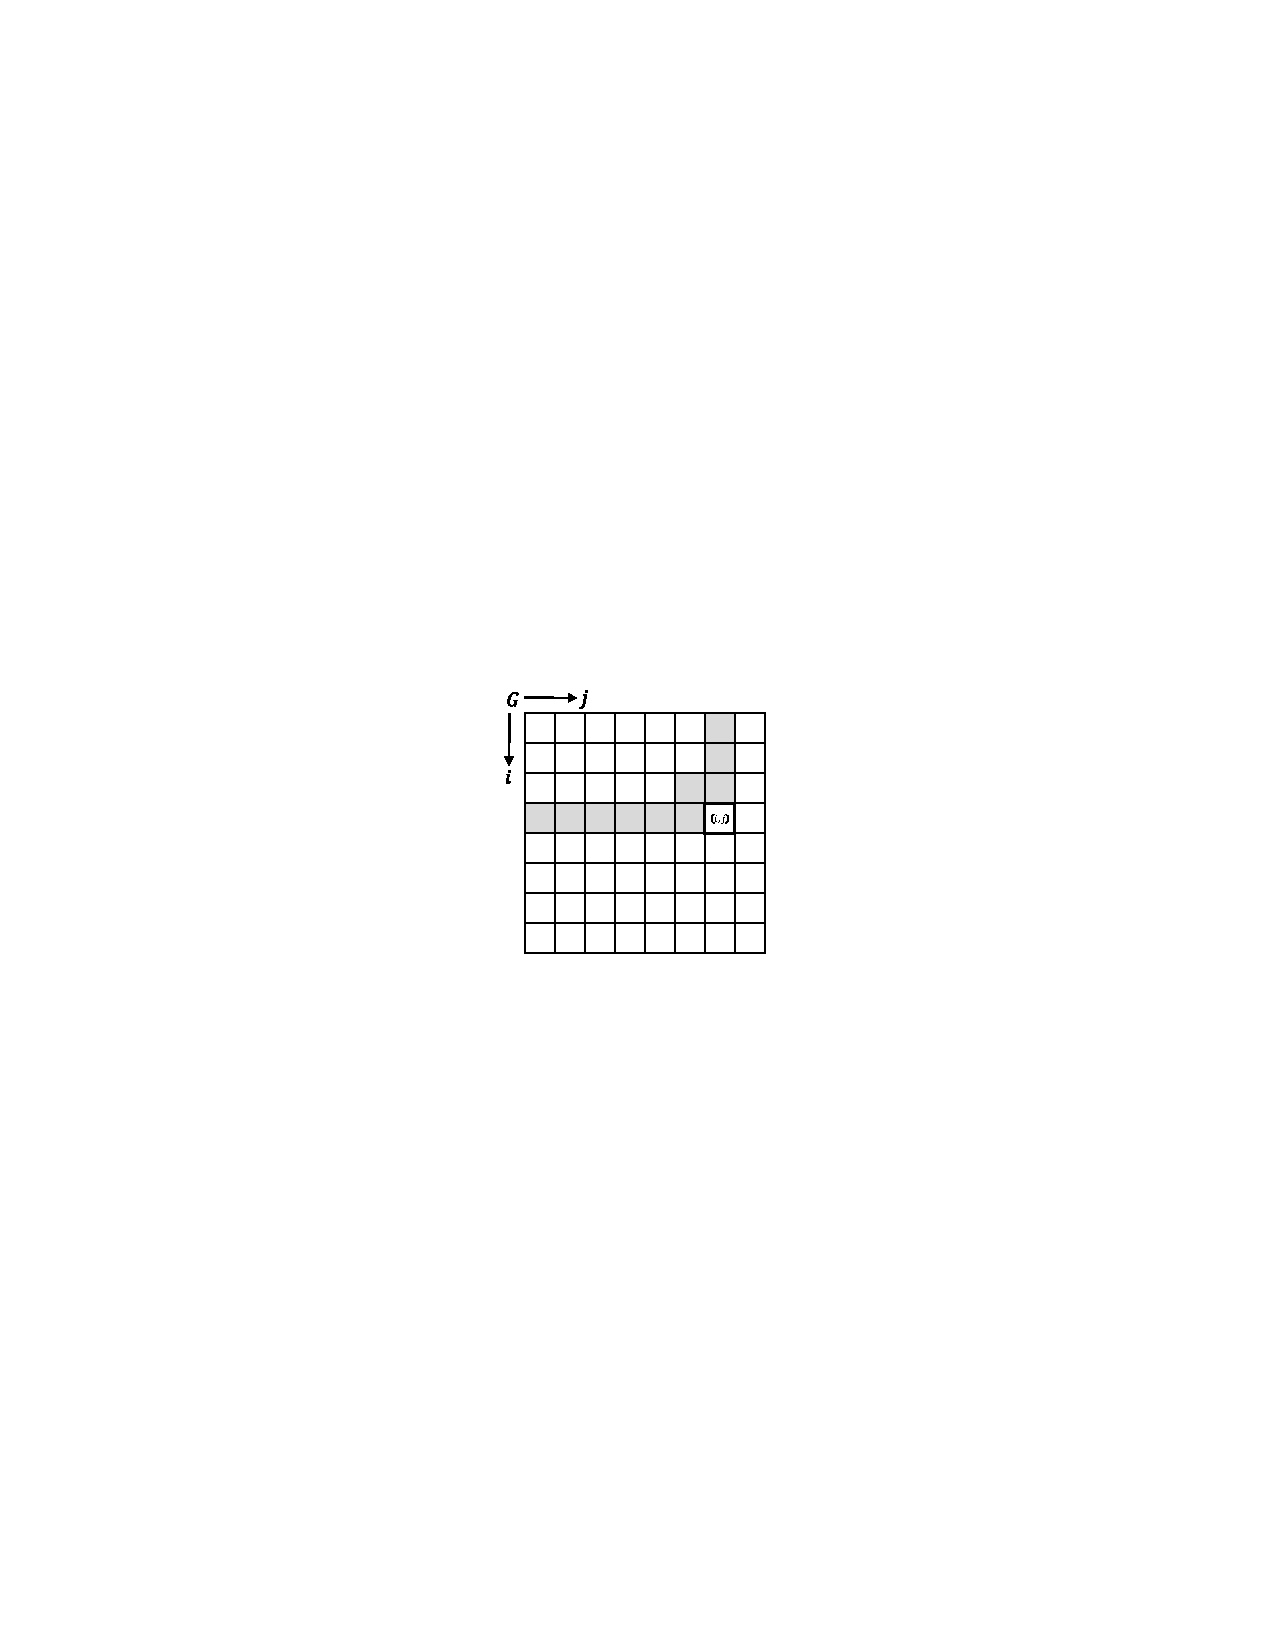
\includegraphics{img/gap-depend}\end{tabular}
\todo{for the simplified version, the cell (i-1,j-1) should not be grayed}
\caption{\label{intro:gap dependency matrix}}
\end{figure}

To address the situation, the algorithm designer would like to separate the parts
of the computation that read from \qbox1 from the parts that read from \qbox2.
This can be achieved here by splitting the $\min_{0\leq(q::K)<j}$ into two
ranges, according to the region in which $G_iq$ resides.

\begin{equation}\LeftEqNo
\renewcommand\arraystretch{1.5}
\begin{array}{l@{}l}
	G_{\,(i :: J_0)\,(j :: K_1)} ~=~  \\
	\qquad
	\begin{cases}
		0                        & i=j=0 \\
		w_{0j}                   & i=0, j>0 \\
		w'_{i0}                  & i>0, j=0 \\
		\begin{array}{@{}l@{~}l}
		  \min\langle & \underset{(q::K_0)}\min ~ G_{iq} + w_{qj}, \\
		              & \underset{(q::K_1) <j}\min ~ G_{iq} + w_{qj}, \\
		              & \underset{0\leq (p::J_0) <i}\min ~ G_{pj} + w'_{pi}~\rangle
		\end{array}              & i,j>0
	\end{cases}
\end{array}
\end{equation}

The path becomes clear: compute $\min_{(q::K_0)} ~ G_{iq} + w_{qj}$ first, for all $i$, $j$
in \qbox2. Then use the results to compute $G_{ij}$.

\begin{equation}\LeftEqNo
\renewcommand\arraystretch{1.5}
\begin{array}{l@{}l}
	G_{\,(i :: J_0)\,(j :: K_1)} ~=~  \\
	\qquad
	\textrm{let}~\psi_{ij} = \underset{(q::K_0)}\min ~ G_{iq} + w_{qj} \\
	\qquad\textrm{in} \\
	\qquad
	\begin{cases}
		0                        & i=j=0 \\
		w_{0j}                   & i=0, j>0 \\
		w'_{i0}                  & i>0, j=0 \\
		\begin{array}{@{}l@{~}l}
		  \min\langle & \psi_{ij}, \\
		              & \underset{(q::K_1) <j}\min ~ G_{iq} + w_{qj}, \\
		              & \underset{0\leq (p::J_0) <i}\min ~ G_{pj} + w'_{pi}~\rangle
		\end{array}              & i,j>0
	\end{cases}
\end{array}
\label{intro:let in 2}
\end{equation}

\medskip
The second part in \eqref{intro:let in 2} starts to look similar to \eqref{intro:gap spec}:
in particular, the types of $p$ and $q$ are the same as those of $i$ and $j$.
In fact, if we set $\psi_{ij}=\infty$, we get \eqref{intro:gap spec} as a special case,
only with $J_0$ and $K_1$ instead of $J$ and $K$.
It therefore makes sense to write a version that generalizes both.

\begin{equation}\LeftEqNo
\renewcommand\arraystretch{1.5}
\begin{array}{l}
	A_{\,\psi\, (i :: J)\, (j :: K)} ~=~  \\
	\qquad
	\begin{cases}
		0                        & i=j=0 \\
		w_{0j}                   & i=0, j>0 \\
		w'_{i0}                  & i>0, j=0 \\
		\begin{array}{@{}l@{~}l}
		  \min\langle & \psi_{ij}, \\
		              & \underset{(q::K)<j}\min ~ A_{\psi iq} + w_{qj}, \\
		              & \underset{(p::J)<i}\min ~ A_{\psi pj} + w'_{pi}~\rangle
		\end{array}              & i,j>0
	\end{cases}
\end{array}
\label{intro:gap phase A}
\end{equation}

\medskip
And we can now rewrite \eqref{intro:gap spec} and \eqref{intro:let in 2} as
%
\begin{equation}
	G_{ij} ~=~ A_{\,(\infty^{JK})\,(i::J)\,(j::K)}
\end{equation}
%
\begin{equation}
\renewcommand\arraystretch{1.3}
\begin{array}{l@{}l}
	G_{\,(i :: J_0)\,(j :: K_1)} ~=~ 
	& \textrm{let}~\psi_{ij} = \underset{(q::K_0)}\min ~ G_{iq} + w_{qj} \\
	& \textrm{in}~A_{\,\psi\,(i::J_0)\,(j::K_1)}
\end{array}	
\label{intro:let in 2 using A}
\end{equation}

\medskip
It takes a bit more insight to notice that \eqref{intro:let in 2 using A} can be further
generalized into:
%
\begin{equation}
\renewcommand\arraystretch{1.5}
\begin{array}{l@{}l}
	A_{\,\psi\,(i :: J)\,(j :: K)} ~=~  \qquad\mbox{(if $i\in J_0$, $j\in K_1$)}\\
	\qquad
	\textrm{let}~\psi'_{ij} = \min \langle~\psi_{ij}, \underset{(q::K_0)}\min ~ G_{iq} + w_{qj}~\rangle \\
	\qquad\textrm{in}~
	A_{\,\psi'\,(i::J_0)\,(j::K_1)}
\end{array}
\label{intro:let in A}
\end{equation}

That is the core of the divide and conquer method: representing the output as a combination
of smaller instances of the problem, or sub-problems, yielding a solution that is essentially
a recursive routine, or a set of mutually recursive routines. In \eqref{intro:let in A}, the
``let''-expression $\psi'_{ij} = \min \langle~\psi_{ij}, \min_{(q::K_0)} ~ G_{iq} + w_{qj}~\rangle$
is another sub-problem that has to be addressed using the same slicing technique.
Once all the pieces fit together, it is possible to cut the space into arbitrarily small pieces,
that fit nicely in each core's local cache. This greately increases performance, as demonstrated
by~\citneeded{perhaps include a table with exact figures}. 

\begin{center}$\vdots$
\end{center}

\subsection{Main Contributions}

\begin{enumerate}
  \item We develop a small set of tactics that can be used to transform a class of recurrence
  specifications intro equivalent divide-and-conquer programs, that admit parallel cache-local
  implementations, in a principled, systematic manner.
  \item We prove that these tactics are semantics-preserving, assuming some side conditions are met
  at the point when the tactic is applied.
  \item We show that the side conditions can be effectively translated into first-order closed
  formulas, and verified automatically by SMT solvers.
\end{enumerate}


\section{Overview}
\label{overview}

Most readers are likely familiar with the Dynamic Programming (DP) technique of Richard Bellman~\cite{03/Bellman:DP} to construct an optimal solution to a problem by combining together optimal solutions to many overlapping sub-problems. The key to DP is to exploit the overlap in order to explore otherwise exponential-sized problem spaces in polynomial time. Dynamic programs are usually described through recurrence relations that specify how the cells in a DP table must be filled using solutions already computed for other cells, but recent research has shown that it is possible to achieve order-of-magnitude performance improvements over this standard implementation approach by developing \emph{divide-and-conquer}  implementation strategies that recursively
partition the space of subproblems into smaller subspaces (see, e.g., \cite{IPDPS15/Tithi}).   For example, Tithi \etal{} have shown that for classical DP problems such as Floyd-Warshall, the parallel divide-and-conquer implementation is  8x faster  across a range of problem sizes compared with a parallel tiled implementation thanks to the better temporal locality and the additional optimization opportunities exposed by partitioning~\cite{IPDPS15/Tithi}. These performance differences matter because  DP is central to many important domains ranging from logistics to computational biology; as an illustrative example, a recent textbook \cite{DurbinEdKr98} on biological sequence analysis lists 11 applications of DP in bioinformatics just in its introductory chapter, with many more in chapters that follow. 

\newcommand{\xidx}{i}
\newcommand{\yidx}{j}
\newcommand{\xw}[1]{w^x_{#1}}
\newcommand{\yw}[1]{w^y_{#1}}

%To set up the premises, we are going to explain how an algorithms expert---we will call him Richard---would go about designing such an implementation by hand.
%We will then show how he will be able to do it more easily using Bellmania.

To illustrate the key concepts undelying Bellmania, we will walk through the first
few steps that an algorithms expert --- whom we will call Richard --- would follow to
generate a provably correct divide-and-conquer implementation of a DP algorithm.
As a motivating example, we consider the Simplified Arbiter problem.
Two processes $x$ and $y$ must be scheduled to run $n$ and $m$ seconds,
respectively, on a single processor, using one-second slots.
Execution starts at $t=0$. The cost for scheduling the slots $[a..b)$ of $x$ after
having scheduled slots $[0..c)$ of $y$
is given by $\xw{abc}$, and the cost for schedulting the slots $[a..b)$ of $y$
after scheduling $[0..c)$ of $x$ is given by $\yw{abc}$.

\begin{figure}[b]
\begin{tabular}{@{\hspace{-1pt}}r@{~}l@{}}
\begin{tikzpicture}[x=4.1mm,y=4.1mm,baseline=(center), remember picture]
  \coordinate(center) at (3,3);
  \draw[step=1] (0,0) grid (6,6);
  \draw[ultra thick] (4,2) rectangle +(1,1);
  %\node(Gij) at (4.5,2.5) {\tiny $\scriptscriptstyle\langle i,j\rangle$};
  \node[circle,fill=BrickRed,inner sep=0,minimum size=1mm](Gij) at (4.5,2.5) {};
  \fill[black,opacity=0.1] (0,5) rectangle (6,6);
  \fill[black,opacity=0.1] (0,0) rectangle (1,5);
  \fill[blue,opacity=0.2] (0,2) rectangle (4,3);
  \fill[blue,opacity=0.2] (4,3) rectangle (5,6);
  \node[anchor=south east](G) at (0,6) {\small$G$};
  \draw[->] (G.east) -- +(1.5,0) node[anchor=west] {\small $j$};
  \draw[->] (G.south) -- +(0,-1.5) node[anchor=north] {\small $i$};
\end{tikzpicture}
&
\small
$
\begin{array}{l@{}}
	\tikz[overlay, remember picture]{\draw[BrickRed] (0,0) -- (Gij);}
	G_{ij} ~=~ \\
	~
	\begin{cases}
		0                        & i=j=0 \\
		\yw{0j0}                  & i=0, j>0 \\
		\xw{0i0}                 & i>0, j=0 \\
		\begin{array}{@{}l@{\hspace{-1pt}}l@{\hspace{-4pt}}}
		  \min\langle & \underset{0\leq q<j}\min ~ G_{iq} + \yw{qji},  \\
		              & \underset{0\leq p<i}\min ~ G_{pj} + \xw{pij}~\rangle
		\end{array}              & i,j>0
	\end{cases}
\end{array}
$
\end{tabular}
\vspace{5pt}
\caption{Recurrence equation and cell-level dependencies.}
\label{overview:arbiter spec}
\end{figure}


The optimal cost for scheduling the first $i$ slots of $x$ and the first $j$ slots
of $y$ is given by the recurrence $G_{ij}$ in \Cref{overview:arbiter spec}. When $i$ is zero, it means that
only $y$ has been scheduled, so the cost is $\yw{0j0}$, and similarly when $j$ is zero, 
the cost is $\xw{0i0}$. When $i$ and $j$ are both positive, there are two options:
either the schedule ends with an allocation to $x$, 
where slots $[p..i)$ of $x$ were scheduled at $t=p+j$, and the cost is 
$G_{pj} + \xw{pij}$; or it ends with an allocation to $y$, where
slots $[q..j)$ of $y$ were scheduled at $t=i+q$, and the cost is $G_{iq} + \yw{qji}$.
The minimum over all respective $p<i$ and $q<j$ is taken.
Eventually, the optimal cost of the entire schedule is given by $G_{nm}$.

\begin{paragraph}{Iterative Algorithm.}
Using a standard dynamic programming method, our algorithm expert Richard would compute this recurrence
with an iterative program by understanding the dependency pattern:
to compute the $\min\langle\cdots\rangle$ expression in \Cref{overview:arbiter spec} and find the optimal
values for $p$ and $q$, the algorithm needs information from all cells above and to the left of $G_{ij}$.
In particular, each value $G_{ij}$ is computed from other values $G_{i'j'}$ with lower
indexes, $i'<i$, ~$j'<j$. 
Therefore, considering $G$ as a two-dimensional array, it can be filled in a single pass from left to right and from top
to bottom, as shown in \Cref{overview:iterative}.
\end{paragraph}

\newcommand\FORLINE[1]{\State\algorithmicfor~{#1} \algorithmicdo~}
\newcommand\Head[1]{\Comment{ {\it #1} ~~}}

\begin{algorithm}
\renewcommand\arraystretch{1.3}
\begin{algorithmic}
  \State $G_{00} := 0$    \Head{Initialize}
  \FORLINE{$i=1..n$}  $G_{i0} := \xw{0i0}$
  \FORLINE{$j=1..m$}  $G_{0j} := \yw{0j0}$  
  \For{$i=1..n$}          \Head{Compute}
    \For{$j=1..m$}
      \State $G_{ij} :=
        \begin{array}[t]{@{}l@{~}l} 
          \min\langle & \underset{0\leq q<j}\min ~ G_{iq} + \yw{qji}, \\
                      & \underset{0\leq p<i}\min ~ G_{pj} + \xw{pij}~\rangle \\         
        \end{array}$
    \EndFor
  \EndFor
\end{algorithmic}
\caption{\label{overview:iterative}
   Iterative Simplified Arbiter}
\end{algorithm}



\newcommand\qbox[1]{\fbox{\rm\scriptsize#1}}
\newcommand\tinyqbox[1]{\hspace{.5pt}\tikz \node[draw,inner sep=1.5pt] {$\scriptscriptstyle #1$};}

\newcommand\plusoneocd{\raisebox{.5pt}{$\scriptstyle+1$}}

\algrenewtext{Procedure}{\hspace{-3mm}{\bf procedure}~}  % hach to make proc header slighly less indented

\begin{paragraph}{Divide-and-Conquer Algorithm.}

\begin{figure}
\centering
\begin{tabular}{c@{\hspace{.5in}}c}
\begin{tikzpicture}[baseline=(n/2), q/.style={font=\relsize{1.3}}]
  \draw (0,0) grid (2,2);
  \node[q] at (.5,1.5) {1};   \node[q] at (1.5,1.5) {2};
  \node[q] at (.5, .5) {3};   \node[q] at (1.5, .5) {4};
  \node(O)[above left] at (0,2) {$0$};
  \node(m/2)[above] at (1,2) {$\frac{m}{2}$};
  \node(m)[above] at (2,2) {$m$};
  \node(n/2)[left] at (0,1) {$\frac{n}{2}$};
  \node(n)[left] at (0,0) {$n$};
  \node(J0)[above] at (.5,2.5) {$J_0$};
  \node(J1)[above] at (1.5,2.5) {$J_1$};
  \node(I0)[left] at (-.5,.5) {$I_0$};
  \node(I1)[left] at (-.5,1.5) {$I_1$};
  %\coordinate(0) at (0,0);
  %\coordinate(sw) at (0,0);
  %\coordinate(ne) at (2,2);
  %\draw (J0.north -| sw) -- node[above] {$J$} ++(ne |- 0);
  %\draw (I0.west |- sw) -- node[left] {$I$} ++(ne -| 0);
  \draw (O.north east) -- (O.north east -| m/2.north west);
  \draw (O.north east -| m.110) -- (O.north east -| m/2.north east);
  \draw (O.south west) -- (O.south west |- n/2.north west);
  \draw (O.south west |- n.160) -- (O.south west |- n/2.220);
\end{tikzpicture}
& 
$\begin{array}{l}\qbox1 \rightsquigarrow \qbox2 \\ 
\qbox1 \rightsquigarrow \qbox3 \\ \qbox2\rightsquigarrow \qbox4 \\ \qbox3 \rightsquigarrow \qbox4\end{array}$
\end{tabular}
\vspace{5pt}
\caption{\label{overview:quadrants}
  Dividing a two-dimensional array into quadrants; the dependencies are shown on the right.}
\end{figure}

Divide-and-conquer is a common algorithm development pattern (\cite{09/CLRS}, chapter 4) that has recently
been applied to DP (\cite{SODA06/Chowdhury,SPAA08/Chowdhury,TOCS10/Chowdhury,TCBB10/Chowdhury}).
This approach has the benefit of yielding cache-oblivious implementations by
increasing memory locality while preserving parallelism. With divide-and-conquer,
the DP table is partitioned into regions, and each region is expressed as a sub-problem
to be solved.

We will now describe how Richard approaches the running example using Bellmania.
He would like to partition the two-di\-men\-sio\-nal array $G$ into
quadrants, as illustrated in \Cref{overview:quadrants}.
In Bellmania, this is accomplished by applying the {\sf Slice} tactic,
illustrated graphically at the top of \Cref{overview:slice-stratify-synth}.
{\em Tactics} are transformation steps that manipulate the program,
and represent a high-level refinement concept.
The partitions are labeled $I_0,I_1$ and $J_0,J_1$ for row index ranges and column index ranges,
respectively.
Slicing gives the analog of the specification in \Cref{overview:logical-slice-stratify}({\it i}).
The expression inside $\min\langle\cdots\rangle$ is shortened for space,
but it is the same as in \Cref{overview:iterative}.

Following the same reasoning as in the iterative case, computing \qbox1
does not depend on any of the other computations. Richard applies the
{\sf Stratify} tactic, which encodes exactly this intuition: it separates
an independent computation step as a separate loop.
This is equivalent to rewriting the specification as in \Cref{overview:logical-slice-stratify}({\it ii}):
the first computation is given a special name $G^{\tinyqbox1}$, then the following
computations read data either from $G^{\tinyqbox1}$ (when the indices are in \qbox1)
or from $G$ (otherwise), which is denoted by $G^{\tinyqbox1}\!/G$. The ``$/\,$'' operator
is part of the Bellmania language and will be defined formally in \Cref{lang}.
Bellmania checks the data dependencies and verifies that the transformation
is sound.

Repeating {\sf Stratify} would result in a four-step computation
as seen in \Cref{overview:chain}, from which Richard can obtain the program in \Cref{overview:breakdown}
(only the first two steps are shown; remaining steps are analogous).
This already gives some performance gain, since the compututations \qbox2 and \qbox3
can now run in parallel. However, this is not what Richard wants; so he
changes the development of this procedure, which he calls ``A'', to produce
a recursive divide-and-conquer algorithm.
\end{paragraph}


\begin{figure}
\[\renewcommand\arraystretch{1.3}
  \begin{array}{@{}l@{}}
    \textsf{Slice} \quad i:\langle I_0|I_1\rangle \quad j:\langle J_0|J_1\rangle \hfill (i)\\
    ~\forall i,j\in\qbox1.~ G_{ij} = \min \langle\cdots G_{iq} \cdots G_{pj} \cdots \rangle \\
    ~\forall i,j\in\qbox2.~ G_{ij} = \min \langle\cdots G_{iq} \cdots G_{pj} \cdots \rangle \\
    ~\forall i,j\in\qbox3.~ G_{ij} = \min \langle\cdots G_{iq} \cdots G_{pj} \cdots \rangle \\
    ~\forall i,j\in\qbox4.~ G_{ij} = \min \langle\cdots G_{iq} \cdots G_{pj} \cdots \rangle \\
    %
    \textsf{Stratify} ~ \qbox1 \hfill (ii)\\
    %
    ~\forall i,j\in\qbox1.~ G^{\tinyqbox1}_{ij} = \min \langle\cdots G^{\tinyqbox1}_{iq} \cdots G^{\tinyqbox1}_{pj} \cdots \rangle \\
    ~\forall i,j\in\qbox2.~ G_{ij} = \min \langle\cdots (G^{\tinyqbox1}\!/G)_{iq} \cdots (G/G^{\tinyqbox1})_{pj} \cdots \rangle \\
    ~\forall i,j\in\qbox3.~ G_{ij} = \min \langle\cdots (G/G^{\tinyqbox1})_{iq} \cdots (G/G^{\tinyqbox1})_{pj} \cdots \rangle \\
    ~\forall i,j\in\qbox4.~ G_{ij} = \min \langle\cdots (G/G^{\tinyqbox1})_{iq} \cdots (G/G^{\tinyqbox1})_{pj} \cdots \rangle
  \end{array}
\]
\caption{\label{overview:logical-slice-stratify}
  The first two steps in the development, represented as logical specifications.}
\end{figure}


\newcommand\steparrowwidth{3mm}
\newcommand\steparrow{
\includegraphics[width=\steparrowwidth]{img/arrow}}

\begin{figure}
\centering
\ifarmando
\bigskip(missing figure)\bigskip
\else
\begin{tikzpicture}[>=latex,x=6mm,y=6mm,
    every path/.style={step=1},
    every node/.style={inner sep=.5pt},
    init data/.style={pattern=horizontal lines, pattern color=green!50!black},
    block/.style={rectangle,draw,very thick,fill=Orange, fill opacity=0.2, inner sep=0}]
    
  \def\dx{1.75cm}
    
  \fill[init data] (0,2) -- ++(.2,0) -- (2,.2) -- (2,0);
  \draw (0,0) grid (2,2);
  \node(s)[block,fit={(0,1) (1,2)}] {};
  %\node(1) at (.5,1.5) {1};   \node(2) at (1.5,1.5) {2};
  %\node(3) at (.5,.5) {3};    \node(4) at (1.5,.5) {4};

  \node[inner sep=0] at (2.5,1) {\steparrow};

  \tikzset{xshift=\dx}
  
  \draw (0,0) grid (2,2);
  \node(1) at (.5,1.5) {1};   %\node(2) at (1.5,1.5) {2};
  %\node(3) at (.5,.5) {3};         \node(4) at (1.5,.5) {4};
  \draw (s.70) edge[->,out=20] (1);
  \node(s)[block,fit={(1,0) (2,1)}] {};
  \node[inner sep=0] at (2.5,1) {\steparrow};

  \tikzset{xshift=\dx}
  
  \draw (0,0) grid (2,2);
  \node(1) at (.5,1.5) {1};  %\node(2) at (1.5,1.5) {2};
                             \node(4) at (1.5,.5) {4};
  \draw (s.-70) edge[->,out=-20,in=-135] (4);
  \fill[block] (0,2) |- (.85,1) to[out=0,in=90] (1,.85) |- (2,0) |- (1.15,1) to[out=180,in=-90] (1,1.15) |- cycle;
  \coordinate(s) at (1.8,0);
  \node[inner sep=0] at (2.5,1) {\steparrow};

  \tikzset{xshift=\dx}
  
  \draw (0,0) grid (2,2);
  \node(1) at (.5,1.5) {1};   \node(2) at (1.5,1.5) {2};
                              \node(4) at (1.5,.5) {4};
  \draw (s.south) edge[->,out=-40,in=-130] (2.-120);
  \coordinate (s) at (.8,0);

\end{tikzpicture}

\fi
\caption[caption]{\label{overview:chain}
  Stratified computation for Simplified Arbiter. \\[.2em]
  The array is initially empty except for the hatched area that is
  filled by {\it Initialize}.
  Shaded areas indicate the region that is read at each step.
  The arrows point at the quadrant that is written to. }
\end{figure}

\newcommand\applytactic[1]{{\tt >} \sf #1}
\newcommand\applytacticnode[1]{\node[right,align=left] at (3,1) {\applytactic{#1}}}


\begin{algorithm}
\renewcommand\arraystretch{1.3}
\begin{algorithmic}
\Procedure{A{\larger{[}}$G${\larger{]}}}{}\EndProcedure
  \For{$i=1..\frac{n}{2}$}    \Head{Compute \qbox1}
    \For{$j=1..\frac{m}{2}$} 
      \State \hspace{-.5cm}$G_{ij} :=
        \begin{array}{@{}l@{~}l} 
          \min\langle & \underset{0\leq q<j}\min ~ G_{iq} + \yw{qji}, 
                        \underset{0\leq p<i}\min ~ G_{pj} + \xw{pij}~\rangle \\         
        \end{array}$
    \EndFor
  \EndFor
  \For{$i=1..\frac{n}{2}$}    \Head{Compute \qbox2}
    \For{$j=\frac{m}{2}\plusoneocd..m$}
      \State \hspace{-.5cm}$G_{ij} :=
        \begin{array}[t]{@{}l@{~}l} 
          \min\langle & \underset{0\leq q<j}\min ~ G_{iq} + \yw{qji}, 
                        \underset{0\leq p<i}\min ~ G_{pj} + \xw{pij}~\rangle \\         
        \end{array}$
    \EndFor
  \EndFor
  \State $\vdots$ \Head{Compute \qbox3}
\end{algorithmic}
\caption{\label{overview:breakdown}
   Simplified Arbiter --- Sliced and Stratified}
\end{algorithm}

\begin{algorithm}
\renewcommand\arraystretch{1.3}
\begin{algorithmic}
\Procedure{A{\larger{[}}$G${\larger{]}}}{}\EndProcedure
  \State A\big[$G_{(0..\frac{n}{2})(0..\frac{m}{2})}$\big] \Head{Compute \qbox1}
  \For{$i=1..\frac{n}{2}$}    \Head{Compute \qbox2}
    \For{$j=\frac{m}{2}\plusoneocd..m$}
      \State $G_{ij} :=
        \begin{array}[t]{@{}l@{~}l} 
          \min\langle & \underset{0\leq q<\frac{m}{2}}\min ~ G_{iq} + \yw{qji}~\rangle \\         
        \end{array}$
          \Comment{(left)}
    \EndFor
  \EndFor
  \For{$i=1..\frac{n}{2}$}
    \For{$j=\frac{m}{2}\plusoneocd..m$}
      \State $G_{ij} :=
        \begin{array}[t]{@{}l@{~}l} 
          \min\langle G_{ij}, & \underset{\frac{m}{2}\leq q<j}\min ~ G_{iq} + \yw{qji}, \\
                      & \underset{0\leq p<i}\min ~ G_{pj} + \xw{pij}~\rangle \\         
        \end{array}$
          \Comment{(right)}
    \EndFor
  \EndFor
  \State $\vdots$
\end{algorithmic}
\caption{\label{overview:further-breakdown}
   Simplified Arbiter --- Sliced Even More}
\end{algorithm}


\newbox\primebox
\setbox\primebox\hbox{$'$}
\newbox\doubleprimebox
\setbox\doubleprimebox\hbox{$''$}

\newcommand\primeocd[1]{\hspace{\wd\primebox}#1\usebox\primebox}
\newcommand\doubleprimeocd[1]{\hspace{\wd\doubleprimebox}#1\usebox\doubleprimebox}

\begin{figure}
\centering
\ifarmando
\bigskip(missing figure)\bigskip
\else
\begin{tikzpicture}[>=latex,x=6mm,y=6mm,
    every path/.style={step=1},
    every node/.style={inner sep=.5pt},
    init data/.style={pattern=north west lines, pattern color=green!50!black},
    block/.style={rectangle,draw,very thick,fill=Orange, fill opacity=0.2, inner sep=0},
    knob/.style={midway,draw,fill=white,midway,inner sep=1.25pt}]
    
  \def\dx{1.75cm}
  \def\dy{1.75cm}
  
  % -------------------------------------------------------

  \draw (0,0) rectangle (2,2);
  \node(s)[block,fit={(0,0) (2,2)}] {};
  \node[inner sep=3mm](0) at (1,1) {0};

  \node[inner sep=0] at (2.5,1) {\steparrow};

  \tikzset{xshift=\dx}

  \draw (0,0) rectangle (2,2);
  \node[inner sep=3mm](0) at (1,1) {0$'$};
  \draw (s.70) edge[->,out=20] (0);

  \applytacticnode{Slice ~~ $i : \langle I_0|I_1\rangle$ ~~ $j : \langle J_0|J_1\rangle$};

  \tikzset{yshift=-\dy,xshift=-\dx}
    
  % -------------------------------------------------------

  \draw (0,0) grid (2,2);
  \node(1) at (.5,1.5) {1};   \node(2) at (1.5,1.5) {2};
  \node(3) at (.5, .5) {3};   \node(4) at (1.5, .5) {4};
  \node(s)[block,fit={(0,0) (2,2)}] {};

  \node[inner sep=0] at (2.5,1) {\steparrow};

  \tikzset{xshift=\dx}

  \draw (0,0) grid (2,2);
  \node(1) at (.5,1.5) {\primeocd 1};   \node(2) at (1.5,1.5) {\primeocd 2};
  \node(3) at (.5, .5) {\primeocd 3};   \node(4) at (1.5, .5) {\primeocd 4};
  \draw (s.70) edge[->,out=20] (1);
  \draw (s.70) edge[->,out=20] (2);
  \draw (s.70) edge[->,out=20] (3);
  \draw (s.70) edge[->,out=20] (4);

  \applytacticnode{Stratify \qbox1};

  % -------------------------------------------------------
  \setlength\baselineskip{15pt}  

  \tikzset{yshift=-\dy,xshift=-\dx}

  \draw (0,0) grid (2,2);
  \node(s)[block,fit={(0,1) (1,2)}] {};
  \node(1) at (.5,1.5) {1};   \node(2) at (1.5,1.5) {2};
  \node(3) at (.5, .5) {3};   \node(4) at (1.5, .5) {4};

  \node[inner sep=0] at (2.5,1) {\steparrow};

  \tikzset{xshift=\dx}
  
  \draw (0,0) grid (2,2);
  \node(1) at (.5,1.5) {\primeocd 1};   \node(2) at (1.5,1.5) {2};
  \node(3) at (.5, .5) {3};             \node(4) at (1.5,.5) {4};
  \draw (s.70) edge[->,out=20] node[knob,circle] {} (1);
  \node(s)[block,fit={(0,0) (2,2)}] {};
  
  \node[inner sep=0] at (2.5,1) {\steparrow};

  \tikzset{xshift=\dx}

  \draw (0,0) grid (2,2);
  \node(1) at (.5,1.5) {\primeocd 1};   \node(2) at (1.5,1.5) {\primeocd 2};
  \node(3) at (.5, .5) {\primeocd 3};   \node(4) at (1.5, .5) {\primeocd 4};
  \draw (s.70) edge[->,out=20] (2);
  \draw (s.70) edge[->,out=20] (3);
  \draw (s.70) edge[->,out=20] (4);
  
  \applytacticnode{Synth $\circ ~~ \dashrightarrow A^{I_0J_0}$ \\ 
      \applytactic{Stratify \qbox2}};
  
  \tikzset{yshift=-\dy,xshift=-2*\dx}

  % -------------------------------------------------------

  \draw (0,0) grid (2,2);
  \node(s)[block,fit={(0,1) (1,2)}] {};
  \node(1) at (.5,1.5) {1};   \node(2) at (1.5,1.5) {2};
  \node(3) at (.5, .5) {3};   \node(4) at (1.5, .5) {4};

  \node[inner sep=0] at (2.5,1) {\steparrow};

  \tikzset{xshift=\dx}
  
  \draw (0,0) grid (2,2);
  \node(1) at (.5,1.5) {\primeocd 1};   \node(2) at (1.5,1.5) {2};
  \node(3) at (.5, .5) {3};   \node(4) at (1.5, .5) {4};
  \draw (s.70) edge[->,out=20] node[knob,circle] {} (1);
  \node(s)[block,fit={(0,1) (2,2)}] {};
  \node[inner sep=0] at (2.5,1) {\steparrow};

  \tikzset{xshift=\dx}
  
  \draw (0,0) grid (2,2);
  \node(1) at (.5,1.5) {\primeocd 1};  \node(2) at (1.5,1.5) {\primeocd 2};
  \node(3) at (.5,.5) {3};             \node(4) at (1.5,.5) {4};
  \draw (s.70) edge[->,out=20] (2);
  \node[inner sep=0] at (2.8,1) {$\cdots$};

  \tikzset{xshift=.25*\dx}

  \node[right,align=left] at (3,1) {\applytactic{Slice \qbox2 \\ \quad $p : \langle J_0|J_1\rangle$}};

  \tikzset{yshift=-\dy,xshift=-2.25*\dx}

  % -------------------------------------------------------

  \draw (0,0) grid (2,2);
  \node(s)[block,fit={(0,1) (1,2)}] {};
  \node(1) at (.5,1.5) {1};   \node(2) at (1.5,1.5) {2};
  \node(3) at (.5, .5) {3};   \node(4) at (1.5, .5) {4};

  \node[inner sep=0] at (2.5,1) {\steparrow};

  \tikzset{xshift=\dx}
  
  \draw (0,0) grid (2,2);
  \node(1) at (.5,1.5) {\primeocd 1};   \node(2) at (1.5,1.5) {2};
  \node(3) at (.5, .5) {3};   \node(4) at (1.5, .5) {4};
  \draw (s.70) edge[->,out=20] node[knob,circle] {} (1);
  \node(s1)[block,fit={(0,1) (1,2)}] {};
  \node(s2)[block,fit={(1,1) (2,2)}] {};
  
  \node[inner sep=0] at (2.5,1) {\steparrow};

  \tikzset{xshift=\dx}
  
  \draw (0,0) grid (2,2);
  \node(1) at (.5,1.5) {\primeocd 1};  \node(2) at (1.5,1.5) {\primeocd 2};
  \node(3) at (.5,.5) {3};             \node(4) at (1.5,.5) {4};
  \draw (s1.70) edge[->,out=20] (2);
  \draw (s2.70) edge[->,out=20] (2);
  \node[inner sep=0] at (2.8,1) {$\cdots$};

  \tikzset{xshift=.25*\dx}

  \node[right,align=left] at (3,1) {\applytactic{Stratify \qbox2$^{\# 1}$}};

  \tikzset{yshift=-\dy,xshift=-2.25*\dx}

  % -------------------------------------------------------

  \draw (0,0) grid (2,2);
  \node(s)[block,fit={(0,1) (1,2)}] {};
  \node(1) at (.5,1.5) {1};   \node(2) at (1.5,1.5) {2};
  \node(3) at (.5, .5) {3};   \node(4) at (1.5, .5) {4};

  \node[inner sep=0] at (2.5,1) {\steparrow};

  \tikzset{xshift=\dx}
  
  \draw (0,0) grid (2,2);
  \node(1) at (.5,1.5) {\primeocd 1};   \node(2) at (1.5,1.5) {2};
  \node(3) at (.5, .5) {3};   \node(4) at (1.5, .5) {4};
  \draw (s.70) edge[->,out=20] node[knob,circle] {} (1);
  \node(s)[block,fit={(0,1) (1,2)}] {};
  
  \node[inner sep=0] at (2.5,1) {\steparrow};

  \tikzset{xshift=\dx}
  
  \draw (0,0) grid (2,2);
  \node(1) at (.5,1.5) {\primeocd 1};  \node(2) at (1.5,1.5) {\primeocd 2};
  \node(3) at (.5,.5) {3};             \node(4) at (1.5,.5) {4};
  \draw (s.70) edge[->,out=20] node[knob,isosceles triangle,rotate=90] {} (2);
  \node(s)[block,fit={(1,1) (2,2)}] {};

  \node[inner sep=0] at (2.5,1) {\steparrow};

  \tikzset{xshift=\dx}
  
  \draw (0,0) grid (2,2);
  \node(1) at (.5,1.5) {\primeocd 1};  \node(2) at (1.5,1.5) {\doubleprimeocd 2};
  \node(3) at (.5,.5) {3};             \node(4) at (1.5,.5) {4};
  \draw (s.70) edge[->,out=20] node[knob,diamond] {} (2);
  \node[inner sep=0] at (2.8,1) {$\cdots$};

  \tikzset{xshift=-1.25*\dx,yshift=-.75*\dy}

  \applytacticnode{Synth {\tikz\node[knob,isosceles triangle,rotate=90] {};} $~~ \longrightarrow B^{I_0J_0J_1}$ \\ 
      \applytactic{Synth $\diamond$} $~~ \dashrightarrow A^{I_0J_1}$};

  \tikzset{yshift=-\dy,xshift=-2*\dx}

\end{tikzpicture}

\vspace{-2mm}
\fi
\caption[caption]{\label{overview:slice-stratify-synth}
  Overview of tactic semantics in Bellmania. }
\end{figure}


\medskip
At this point, Richard notices that {\it Compute \qbox1} is just a smaller version of
the original {\it Compute}; so following {\sf Stratify} \qbox1, he invokes {\sf Synth}, which automatically
synthesizes a recursive call A\big[$G_{(0..\frac{n}{2})(0..\frac{m}{2})}$\big]
(presented using abstract index ranges as $A^{I_0J_0}$).

The other steps require some further algebraic manipulation.
Observe that the computation of \qbox2 is {\bf not} equivalent to
A\big[$G_{(0..\frac{n}{2})(\frac{m}{2}..m)}$], 
because when $\frac{m}{2} \leq j < m$, the range $0\leq q < j$ leads to
some accesses $G_{iq}$ lying outside of \qbox2.

Richard addressed this problem by splitting the range of $q$ using the {\sf Slice}
tactic again, effectively breaking the original $\min\langle\cdots\rangle$ into two:
one where $0\leq q < \frac{m}{2}$,
and one where $\frac{m}{2}\leq q < j$. 
He uses {\sf Stratify} to organize the loops in the program such that both 
loops write to the same area, namely \qbox2, where the second loop reads data
written by the first loop, as shown in \Cref{overview:further-breakdown}.
It is important to notice that the first loop only reads from \qbox1, 
while the second loop only reads from \qbox2.

The computation of \qbox2:(right) is now a true copy of A,
with sub-matrix $G_{(0..\frac{n}{2})(\frac{m}{2}..m)}$ (with the small caveat,
that A has to be changed to include the term $G_{ij}$ in the $\min\langle~\rangle$ expression).
Again, Bellmania synthesizes the sub-call and proves the equivalence.
Running {\sf Synth} on \qbox2:(left) will reveal that it is a new computation,
to which Richard gives the name ``B''. 

After repeating
the same reasoning steps to \qbox3 and \qbox4,
Richard finally has the version in \Cref{overview:recursive-A}.
The base case (when $G$ is small) is added automatically by the Bellmania compiler.
The specific size bound needs to be tuned for performance.\footnote{The auto-tuning step is not implemented in the current version.}


\begin{algorithm}
\renewcommand\arraystretch{1.3}
\begin{algorithmic}
\Procedure{A{\larger{[}}$G${\larger{]}}}{}\EndProcedure
  \If{$G$ {\it is very small}} {\it run iterative version}
  \Else
  \State A\big[$G_{(0..\frac{n}{2})(0..\frac{m}{2})}$\big] \Head{Compute \qbox1}
  \State B\big[$G_{(0..\frac{n}{2})(0..\frac{m}{2})}, 
                G_{(0..\frac{n}{2})(\frac{m}{2}..m)}$\big]    \Head{Compute \qbox2}
  \State A\big[$G_{(0..\frac{n}{2})(\frac{m}{2}..m)}$\big]
  \State C\big[$G_{(0..\frac{n}{2})(0..\frac{m}{2})}, 
                G_{(\frac{n}{2}..n)(0..\frac{m}{2})}$\big]    \Head{Compute \qbox3}
  \State A\big[$G_{(\frac{n}{2}..n)(0..\frac{m}{2})}$\big]
  \State B\big[$G_{(\frac{n}{2}..n)(0..\frac{m}{2})}, 
                G_{(\frac{n}{2}..n)(\frac{m}{2}..m)}$\big]    \Head{Compute \qbox4}
  \State C\big[$G_{(0..\frac{n}{2})(\frac{m}{2}..m)}, 
                G_{(\frac{n}{2}..n)(\frac{m}{2}..m)}$\big]
  \State A\big[$G_{(0..\frac{n}{2})(\frac{m}{2}..m)}$\big]
  \EndIf
\end{algorithmic}
\caption{\label{overview:recursive-A}
   Simplified Arbiter --- Recursive Version}
\end{algorithm}

Richard must then use the same strategy to further break down and
transform the computations of B and C, each into four recursive sub-computations, 
further improving the locality of the resulting algorithm.
Eventually, through these transformations, he can succeed in breaking the computation of $G$ into recursive sub-computations leading to a true divide-and-conquer algorithm. 

As is well illustrated by the example, this line of reasoning can get quite complicated for most dynamic programming algorithms, 
and producing a correct divide-and-conquer algorithm for a given dynamic programming problem is considered quite difficult even by the researchers who originally pioneered the technique. 
Fortunately, the reasoning can be mechanized in Bellmania, which allows
Richard and other algorithm designers to produce an implementation of this algorithm
as well as a {\bf machine-checked proof} of correctness
through a series of high-level tactic application.

Overall, it took Richard only about 10 steps to construct \Cref{overview:recursive-A},
and a total of 26 steps to construct all three steps of the Simplified Arbiter,
comprising an implementation that is 10$\times$ faster than a parallel
\Cref{overview:iterative} generated by a state-of-the-art parallelizing compiler.
The user is greatly assisted by tactics like {\sf Synth}, that carry out the monotonic
and error-prone task of choosing the right parameters for each recursive call; also,
mistakes are identified early in the development thanks to automatic verification,
saving hours of debugging later on.

Once a divide-and-conquer algorithm is found, generating an optimal implementation still requires some additional work, such as finding the right point at which to switch to an iterative algorithm to leverage SIMD parallelism as well as low-level tuning and compiler optimization;
these steps are performed by more traditional compiler optimization techniques
as discussed in \Cref{codegen}.

In the following sections, we describe the different components of Bellmania. 
The system utilizes \newterm{solver-aided tactics} to manipulate a given specification
and generate provably correct pseudo-code; 
this approach is demonstrated by engineering specialized tactics for the domain of divide-and-conquer DP.


\bibliographystyle{abbrvnat}
\bibliography{oopsla2016}
% The bibliography should be embedded for final submission.

%\begin{thebibliography}{}
%\softraggedright

%\bibitem[Smith et~al.(2009)Smith, Jones]{smith02}
%P. Q. Smith, and X. Y. Jones. ...reference text...

%\end{thebibliography}


\end{document}
